\chapter{Clustering}

\section{Evaluation of a new instance}

At this point, with a model trained on the data, a generic $n$th new snapshot instance $\mathcal{S}_n$ can be evaluated using the K-means algorithm.
From a geometric point of view, the snapshot $\mathcal{S}_n$ is a point in the $F$-dimensional space, where $F$ is the number of features used to train the model.

For demonstration purposes, in this section, it is considered an example with $3$ features.

\begin{figure}[htbp]
  \centering
  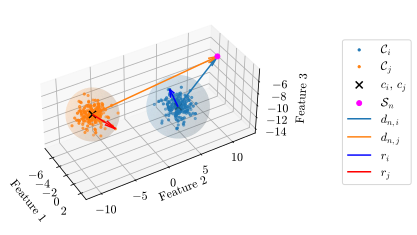
\includegraphics[width=\textwidth]{images/Spheres_2.pdf}
\caption{New instance evaluation}
\label{fig:clust_spheres}
\end{figure}

In the \autoref{fig:clust_spheres}, the training data are represented in the $3$-dimensional space, where the axis are the features used to train the model. The K-means model has been ideally trained with an arbitrary number $k$ of clusters but, for display purposes, only two clusters  ($\mathcal{C}_i$ and $\mathcal{C}_j$) are plotted. 
